%% BEAMER slides (with notes)
%
%
\documentclass[a4paper,12pt]{beamer}
\usepackage{graphicx}
\usepackage{amsmath}
\usepackage{amssymb}
\usepackage{bm}
\usepackage{tikz}
\usepackage{pgfplots}
\title{Approximating price vectors}
\date{\today}
\author{Calvin Roth}
\begin{document}
\maketitle
\begin{frame}
  \frametitle{Introduction}
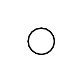
\begin{tikzpicture}
\node[draw,circle,fill=white] (a) at (0,0) {};
\node[draw,circle,fill=white] (b) at (0,0) {};
\node[draw,circle,fill=white] (c) at (0,0) {};
\node[draw,circle,fill=white] (d) at (0,0) {};
\end{tikzpicture}
\end{frame}


\begin{frame}
  \begin{itemize}
    \item Humans are social creatures, our behavior influences other behavior
    \item When our peers engage in a behavior, we are more likely do so as well
          \item CITE SOME OF THE RELEVANT EXAMPLES INCLUDING SOME SEEN IN CLASS
  \end{itemize}
\end{frame}

\begin{frame}
  \begin{itemize}
    \item How to analyze the effect of the social network on consumption \\
    \item We will use the model first proposed by \cite{candogan2012optimal} and later used by \cite{huang2021value} to model an individuals utility u
          \begin{equation}
            u_{i}(x, p) = ax_{i} - x_{i}^{2} + 4 \rho x_{i} \sum \frac{G_{ij}}{\|G+G^{T}\|} x_{j} - p_{i}x_{i}
          \end{equation}
          where $a,\rho$ are constants and $p_{i}$ is the price user i is charged.
\end{itemize}
\end{frame}


\begin{frame}
  \begin{itemize}
    \item A manufacturer who can produce goods at unit price c with $c < a$ wants to maximize profits.
    \item Use network information to charge influencers less and influencees more.
    \item The optimal prices to charge each individual is well understood\cite{candogan2012optimal}\cite{huang2021value}

          \begin{equation}
            \frac{a+c}{2} \textbf{1} + \frac{a-c}{2} \frac{\rho}{\| G + G^{T}\|} (G - G^{T}) K(G+G^{T}, \frac{\rho}{\|G+G^{T}\|})
          \end{equation}
          where $K(X, y) = (I - yX)^{-1}\textbf{1}$, the bonanich centrality vector.
   \end{itemize}
\end{frame}

\begin{frame}
  \begin{itemize}
    \item But we often don't have ready access to the full network information
    \item Given partial enough of the network ex. degrees of network should we do?
    \item Specifically, we want a way to generate a ``good enough'' price vector v with respect to this partial information
          Goal: minimize expected regret
          \begin{equation}
            \mathbb{E} [ 1 - \frac{P_{G}(v)}{Optimal-Profit} | \text{Statistic of G}]
          \end{equation}
          Where $P_{G}(v)$ is the profit of our v on the real network G.
  \end{itemize}
\end{frame}


\begin{frame}
  \frametitle{Degree Seqeunce Information}
  \begin{itemize}
    \item Suppose we are given the degree sequence of the network G(directed graph)
    \item Strategy 1: Make a new graph H with the same degree sequence as G using the configuration model
    \item Hypothesis: H behaves like G so maybe the optimal price vector of H is close to the optimal price vector of G
          \item It is not obvious that local properties of the network should strongly impact global properties(optimal profit)
  \end{itemize}
\end{frame}

\begin{frame}
  \frametitle{Results}
  \begin{itemize}
    \item The answer is yes, this is a strategy to get good price vectors for an unknown graph \\
    \item The following results will show this to be the case
  \end{itemize}
\end{frame}

\begin{frame}
  \frametitle{Details of Testing}
  \begin{itemize}
    \item Generate a graph G with the Erdos-Renyi model with n nodes and link probablity p
    \item Generate either Same Parameter graphs(i.e. same n and p but no further restriction) or Graphs with the same sequence
    \item After we have generated a price vector use G to check how close we were.
    \item Examine experiment various properties of these samples
  \end{itemize}
\end{frame}


\begin{frame}
  \frametitle{Distribution of profits}
  \begin{itemize}
    \item How much more money do we make applying a Same-Sequence price vector than a Same-Parameter to the true graph
  \end{itemize}
\end{frame}

\begin{frame}
  \frametitle{Statistic of distribution of Profits}
  fdafd
\end{frame}



\begin{frame}
  \frametitle{Distribution of Prices}
  \begin{itemize}
    \item The next question to ask is do the same sequence price vectors look like the optimal price vector?
    \item Again the answer is yes
  \end{itemize}
\end{frame}

\begin{frame}
  \frametitle{Statistics of the Prices}
  fada
\end{frame}

\begin{frame}
  \frametitle{A second strategy}
  \begin{itemize}
    \item Above we have shown that the price vector of generated graphs is on average like the optimal price vector
    \item [Strategy 2] The averaged price vector is even more like the optimal price vector
          \begin{equation}
            v = \frac{1}{\# Trials} \sum Profit_{G} (\text{Guessed vector})
          \end{equation}
          \begin{equation}
            v = Profit_G ( \frac{1}{\# Trials} \sum \text{Guessed vector} )
          \end{equation}
  \end{itemize}
\end{frame}

\begin{frame}
  \frametitle{Results}
\end{frame}


\begin{frame}
  \frametitle{Other Directions}
  \begin{itemize}
    \item If knowing the degrees is good then maybe knowing $[|N(v)|, |N(N(v))\setminus (N(v) \cup v ) |$ is better\\
    \item i.e. how many nodes can v reach in 1 or 2 steps \\
    \item What about k steps?
  \end{itemize}
\end{frame}

\begin{frame}
  \frametitle{Results for limited walk information}
\end{frame}


\begin{frame}
  \frametitle{Future Work}
  \begin{itemize}
    \item Mathematical Assurances of error in either strategy
    \item Other Network distributions other than Erdos Renyi
  \end{itemize}
\end{frame}

\bibliography{refer}
\bibliographystyle{ieeetr}

\end{document}

